\subsection*{CATboost}
\ \par Catboost is an algorithm based on Gradient Boosting Tree, which is similar to XGboost and LightGBM. However, Catboost can deal with string data type directly, which is a very good characteristic for this problem since we think string attribute like team name or pitcher name are important for training and cannot be dropped. 
\par In all of the following experiment, i use mean of column to replace numerical column's NAN, and use 'NAN' to replace all NANs in string column. 
\par In the initial tries, we use parameters as following
\begin{lstlisting}[language=Python]
iterations = 500, depth = 5, learning_rate = 0.05, loss_function = 'Logloss'
\end{lstlisting}
\par This is our first algorithm that reaches 0.58 in public test. However, it is still not good enough to pass benchmark. 
\par To find a better set of parameters, we use optuna to help us find it. And to mimic to stage1 / stage2 situation we will met, we use following different strategy to cut training and validation test for optuna.
\begin{itemize}
    \item[stage1] Since we are predicting the last half season given each year's first half season, we use the last 0.2 of each season's data as validation data, and other as training data, and feed these to optuna to find the best parameters.
    \item[stage2] We are predicting a whole new year. Hence we take 2023's data as validation data, and other as training data, and feed these to optuna to find best parameters.
\end{itemize}
\begin{figure}[h]
    \centering
    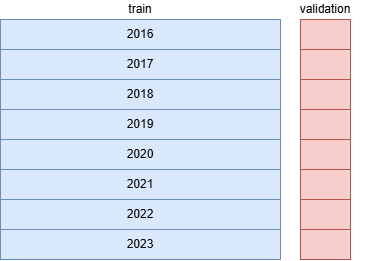
\includegraphics[width=0.25\linewidth]{Pictures/MLdatacut_stage1.drawio.png}
    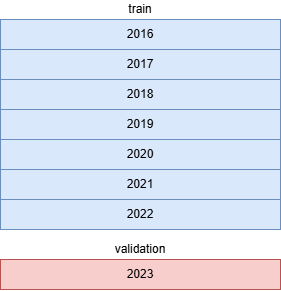
\includegraphics[width=0.17\linewidth]{Pictures/MLdatacut_stage2.drawio.png}
    \caption{Illustrate of our validation cut strategy}
\end{figure}
\par When using optuna, we search in following range
\begin{lstlisting}[language=Python]
params = {
    "iterations": trial.suggest_int("iterations", 100, 1000),
    "depth": trial.suggest_int("depth", 4, 10),
    "learning_rate": trial.suggest_float("learning_rate", 1e-3, 0.3, log=True),
    "l2_leaf_reg": trial.suggest_float("l2_leaf_reg", 1, 10),
    "bagging_temperature": trial.suggest_float("bagging_temperature", 0, 1),
    "random_strength": trial.suggest_float("random_strength", 0.1, 10),
    "loss_function": "Logloss",
}
\end{lstlisting}
The best parameters lead to a 0.57985 accuracy in stage1. And 0.54493 in stage2. Which is not quite stable between two stages. Catboost is a very efficient model, which finish a single round of prediction in a minute. However, doing optuna will take hours to find best parameters (depends on rounds). 
\subsubsection*{Package Reference}
\begin{lstlisting}
optuna, catboost
\end{lstlisting}